\documentclass[12pt, a4paper]{article}
\usepackage{graphicx}
\usepackage[ngerman]{babel}
\usepackage{hyperref}
\usepackage{fontspec}
\usepackage{wrapfig,lipsum}
\usepackage[margin=2cm]{geometry}
\usepackage[export]{adjustbox}
\usepackage{listings}
\usepackage{color}

\lstset{language=Python,
	basicstyle=\scriptsize,
	keywordstyle=\color{red}\bfseries,
	identifierstyle=\color{blue},
	commentstyle=\color{DarkGreen},
	breaklines=true,
	numbers=left,
	numberstyle=\tiny,
	frame=single,
	backgroundcolor=\color{myGrey},
	tabsize=2}
\definecolor{myGrey}{gray}{0.9}
\definecolor{DarkGreen}{rgb}{0.2,0.5,0.6}

\setmainfont{montserrat.ttf}

\graphicspath{{./bilder/}}

\title{Dokumentation des RBG-Sensors \break Fach: ITEC}
\author{Julius Hahl, Maximilian Trautwein und Sebastian Köhler, 11BG1 \\ 
\includegraphics[width=\textwidth]{fbs_logo.pdf}}

\begin{document}
	
	\maketitle
	\newpage
	
	\tableofcontents
	\newpage
	
	\section{Zweck und Einsatzmöglichkeiten}
	\subsection{Zweck}
	Der RGB-Sensor soll Farben erkennen und diese über das lokale/globale Netzwerk schicken. Geräte , die diese Farbinformation brauchen, können eine Funktion aufrufen(auch über ein Event) und somit die Farbe für den derzeitigen Farbwürfel zurückgeben, woraufhin der Roboter seine Tätigkeit fortsetzen kann(zB.: Würfel in das richtige Lager legen).
	\subsection{Einsatzmöglichkeiten}
	Wie im vorherigen Teil schon erwähnt, kann der RGB-Sensor dazu verwendet werden, um einem Roboter beim Einordnen verschiedenfarbiger Gegenstände einzuordnen. Der Sensor fungiert als Auge:
	\\
	\begin{figure}[h]
		\centering
		
		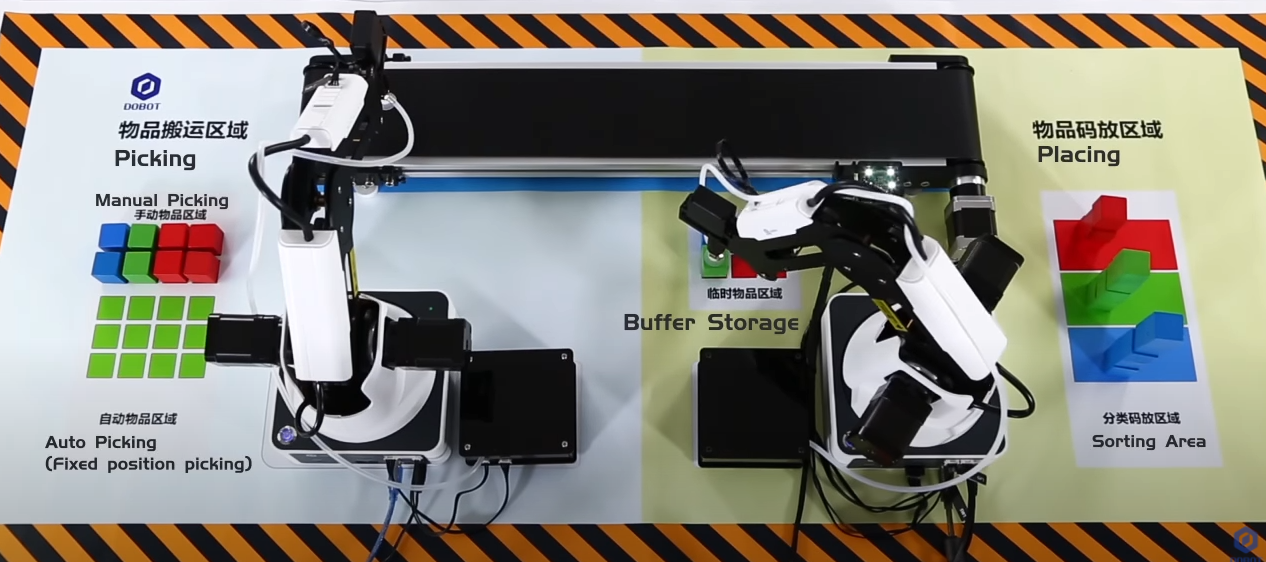
\includegraphics[width=\textwidth, frame]{roboter.png}
		\caption{Beispiel eines Roboterarms beim Sortieren.}
	\end{figure}
	\newpage
	
	\section{Technische Daten}
	\subsection{Hardware}
	\begin{itemize}
		\item Raspberry Pi 4 B 4GB RAM 
		\item Joy-IT Armor Case 
		\item RPi4 Kamera
		\item Standard Raspberry Pi 4 Netzteil
	\end{itemize}

	\begin{figure}[h]
		\centering
		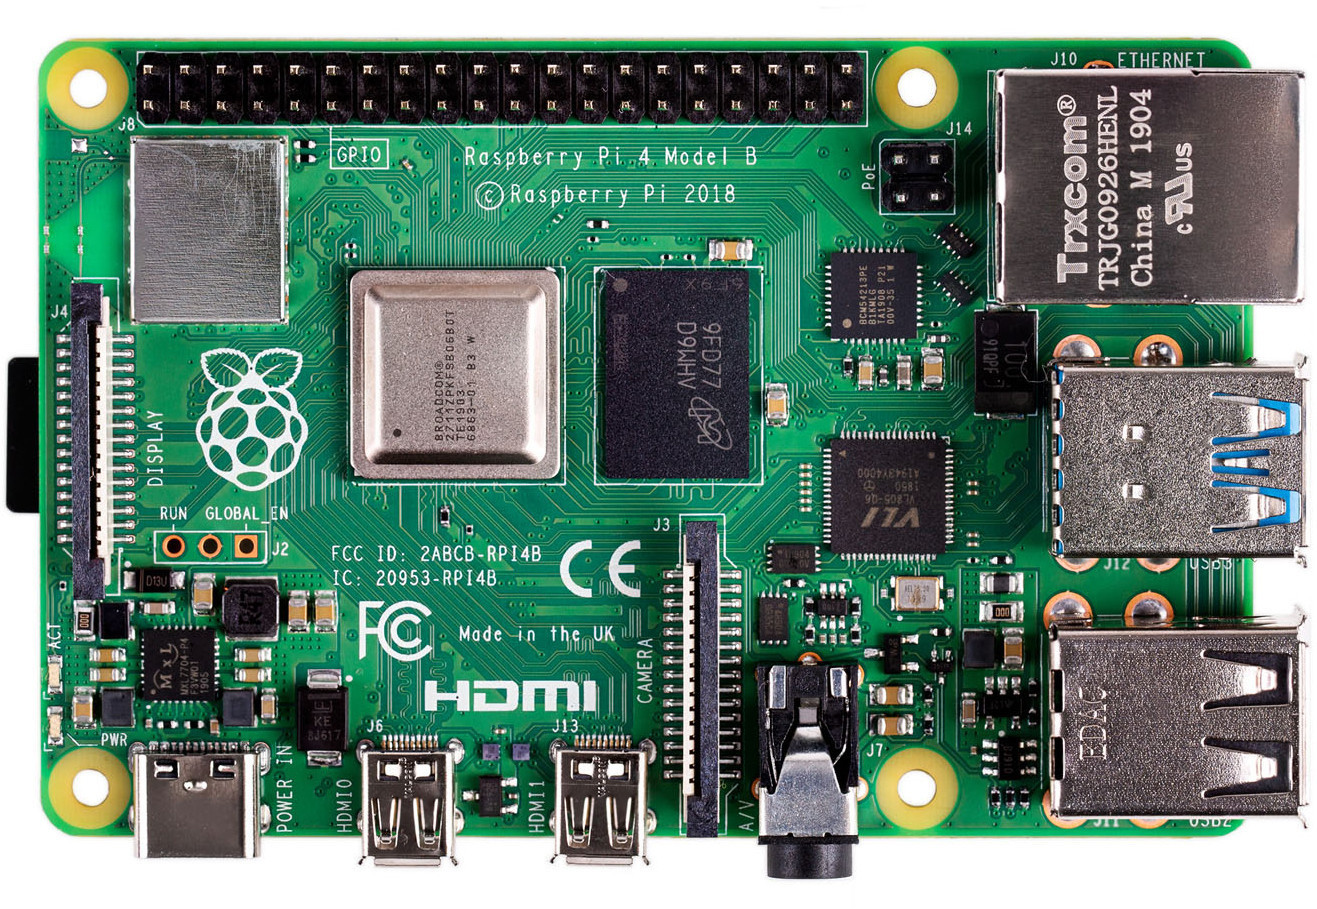
\includegraphics[frame, scale=0.2]{rpi4.jpg}
		\caption{Das Herzstück des Projekts.}
	\end{figure}

	\subsection{Software}
	\begin{itemize}
		\item OpenCV 4.5.5 (Quellcode für 64-Bit kompiliert, \hyperlink{https://opencv.org/}{https://opencv.org/}) 
		\item libcamera Python-Sprachanbindung (nur auf 64-Bit Systemen ausführbar)
		\item Python 3
	\end{itemize}
	\newpage

	\section{Funktionsweise und Beispiel}
	\subsection{Funktionsweise(Quellcode)}
	In dieser Sektion wird der Quellcode nochmals kommentiert dargelegt.
	\lstset{caption={main.py}}
	\begin{lstlisting}
		import cv2 as cv
		import socket
		import sys
		
		from null_preview import *
		from picamera2 import *
		
		#Setup des Sockets und der Kamera
		currentColor = ""
		lastColor = ""
		sock = socket.socket(socket.AF_INET, socket.SOCK_STREAM)
		server_address = (str(sys.argv[1]), 18769)
		print('starting up on {} port {}'.format(*server_address))
		sock.bind(server_address)
		picam2 = Picamera2()
		preview = NullPreview(picam2)
		picam2.configure(picam2.preview_configuration(main={"size":(640, 480)}))
		picam2.start()
		sock.listen(1000)
		connection, client_address = sock.accept()
		
		
		#Bild der Kamera wird als Numpy Array ausgelesen
		def evaluate_current_frame():
		img = picam2.capture_array()
		
		img = cv.cvtColor(img, cv.COLOR_BGR2RGB)
		
		Z = img.reshape((-1,3))
		# Konventiert zu np.float32
		Z = np.float32(Z)
		# Definiton der Kriterien der Farbdominanz, Anzahl an dominanten Farben(K) und anschliessend wird der KMeans Algorithmus angewendet
		criteria = (cv.TERM_CRITERIA_EPS + cv.TERM_CRITERIA_MAX_ITER, 10, 1.0)
		K = 1
		ret,label,center=cv.kmeans(Z,K,None,criteria,10,cv.KMEANS_RANDOM_CENTERS)
		# Zurueck zu unsigned int, damit das Buffer mit dem Bild wieder zu der urspruenglichen Form zurueckkehrt
		center = np.uint8(center)
		res = center[label.flatten()]
		res2 = res.reshape((img.shape))
		
		
		#Trennt Farbkanaele
		(b, g, r) = cv.split(res2)
		
		b_mean = np.mean(b)
		g_mean = np.mean(g)
		r_mean = np.mean(r)
		
		# Bestimmt die prominenteste Farbe und setzt die Variable
		if (b_mean > g_mean and b_mean > r_mean):
		currentColor = "blue"
		elif (g_mean > r_mean and g_mean > b_mean):
		currentColor = "green"
		else:
		currentColor = "red"
		
		#Sendet String an den Client zurueck		
		
		message = currentColor.encode()
		connection.sendall(message)
		
		def close_socket():
		sock.close()
		
		while True:
		try:
		data = connection.recv(16)
		dataBuffer = data.decode('utf-8')
		if(dataBuffer == "getcolor"):
		evaluate_current_frame()
		elif(dataBuffer == "closesocket"):
		close_socket()
		
		
		except OSError:
		print("STOPPED")
		sock.close()
		break
		
		except KeyboardInterrupt:
		print("STOPPED")
		sock.close()
		break
	\end{lstlisting}
	\newpage
	\lstset{caption={client.py}}
	\begin{lstlisting}
		import socket
		import sys
		import tkinter as tk
		
		ip_was_false = True
		
		i = 1
		#Socket definieren
		sock = socket.socket(socket.AF_INET, socket.SOCK_STREAM)
		
		getColorFuncName = "getcolor"
		sockCloseFuncName = "closesocket"
		
		#Funktion zum Verbinden mit dem Raspberry Pi
		def connect_to_server():
		try:
		print(ip_var.get())
		server_address = (ip_var.get(), 18769)
		print('connecting to {} port {}'.format(*server_address))
		sock.connect(server_address)
		except Exception:
		global ip_was_false
		if (ip_was_false == True):
		label2 = tk.Label(root, text = "Falsche IP-Adresse!", fg = '#ff0000')
		label2.pack()
		ip_was_false = False
		
		#Abfrage der derzeitigen Farbe
		def request_color():
		message = getColorFuncName.encode()
		sock.sendall(message)
		
		data = sock.recv(16)
		global i
		lb1.insert(i, data.decode('utf-8'))
		i = i + 1
		
		#Schliessen des Sockets nach Schliessen des Programms
		def close_socket():
		message = sockCloseFuncName.encode()
		sock.sendall(message)
		
		#Definition des Fensters und des Inhalts
		root = tk.Tk()
		root.geometry("250x170")
		
		ip_var = tk.StringVar()
		
		label1 = tk.Label(root, text="RGB-Sensor-System")
		label1.pack()
		
		ip_feld = tk.Entry(root, textvariable = ip_var)
		ip_feld.pack()
		
		schaltf1 = tk.Button(root, text="Verbinde zum Server", command=connect_to_server)
		schaltf1.pack()
		
		schaltf2 = tk.Button(root, text="Farberkennung", command=request_color)
		schaltf2.pack()
		
		lb1 = tk.Listbox()
		
		root.mainloop()
	\end{lstlisting}
	\newpage
	\subsection{Beispiel}
	\subsubsection{Raspberry Pi aufsetzen:}
	Um den Raspberry Pi aufzusetzen, muss man diesen zuerst über ein HDMI-Kabel oder über SSH verbinden, sich 			einloggen (Benutzername: pi, Passwort:ilovecolors) und 
	mit einem Netzwerk verbinden, wo der Laptop/Computer auch angeschlossen ist. Daraufhin kann man die Ausführung 		starten, indem man in der Console des Raspberry Pi's \\ "python main.py *hier die lokale IP-Adresse eingeben*" 		\\ schreibt und auf 'Enter' drückt.
	\begin{figure}[h]
		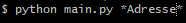
\includegraphics{beispiel.png}
	\end{figure}
	\\
	Jetzt sollte der Raspberry Pi aufgesetzt sein.
	\\
	\subsubsection{Client-Seite (Computer oder Laptop)}
	Wenn der PC im gleichen Netzwerk ist und sie den ersten Schritt vollendet haben, können sie die Python-Datei 		'client.py' ausführen und dort die lokale IP-Adresse des Pi's eingeben und sich verbinden.
	
	\begin{figure}[h]
		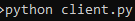
\includegraphics{beispiel2.png}
	\end{figure}
	\noindent	
	!!!Achtung, es ist wichtig, dass sie Python 3 auf ihrem PATH installiert haben und in dem Projektordner sind, 
	damit die Datei ausgeführt werden kann!!! 
	\\
	\\
	Mit dem Knopf 'Verbinden zum Server' verbinden sie sich mit dem Raspberry Pi. Der Knopf 'Farberkennung' schickt eine Anfrage an den Raspberry Pi, der dann die Farbe erkennt und diese dann zurückschickt. Die erkannte 
	Farbe sieht man dann in der Liste.
	
	\begin{figure}[h]
		\centering
		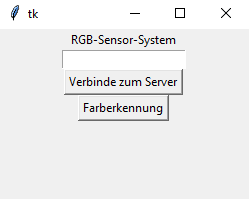
\includegraphics[frame]{clientBeispiel.png}
		\caption{GUI des Programms}
	\end{figure}
	\newpage
	
	\section{Projektphase}
	Wir würden die Projektphase als etwas holprig bezeichnen. Wir sind die einzige Gruppe, die sich für ein 64-Bit-System entschieden haben, um die Effizienz zu steigern. Jedoch mussten wir die neue libcamera-Bibliothek verwenden, sowie OpenCV kompilieren, da die vor-kompilierten Versionen nur für 32-Bit-Systeme vorgesehen sind.  
	\section{Quellen}
	Roboter: \url{https://www.youtube.com/watch?v=AWFFJYYCF44}
	\\
	Raspberry Pi 4: \url{https://www.amazon.de/Raspberry-Pi-ARM-Cortex-A72-Bluetooth-Micro-HDMI/dp/B07TC2BK1X}
	
\end{document}